\documentclass{article}
\input{glyphtounicode}
\pdfgentounicode=1
\usepackage{mlsys2027}
\setcitestyle{numbers,square}
\usepackage[utf8]{inputenc}
\usepackage{amsmath,amssymb,amsfonts,amsthm}
\usepackage{booktabs}
\usepackage{listings}
\lstdefinestyle{structStyle}{
  language=C++,
  basicstyle=\fontsize{5.0pt}{5.8pt}\ttfamily,
  keywordstyle=\bfseries\color{blue!80!black},
  commentstyle=\itshape\color{gray!70!black},
  breaklines=false,
  columns=fullflexible,
  keepspaces=true,
  tabsize=2,
  showstringspaces=false
}
\lstdefinestyle{cudaStyle}{
  language=C++,
  basicstyle=\fontsize{4.2pt}{4.9pt}\ttfamily,
  keywordstyle=\bfseries\color{blue!80!black},
  commentstyle=\itshape\color{gray!70!black},
  breaklines=false,
  columns=fullflexible,
  keepspaces=true,
  tabsize=2,
  showstringspaces=false
}
\usepackage{tabularx}
\usepackage{makecell}
\usepackage{array}
\usepackage{graphicx}
\usepackage{hyperref}
\usepackage{microtype}
\usepackage{xr}
\makeatletter
\let\orig@bibcite\bibcite
\let\bibcite\@gobbletwo
\externaldocument{supplementary}
\let\bibcite\orig@bibcite
\makeatother
\usepackage{xcolor}
\usepackage{multirow}
\usepackage{caption}
\captionsetup{font=small,skip=3pt}

\renewcommand{\topfraction}{0.95}
\renewcommand{\bottomfraction}{0.95}
\renewcommand{\textfraction}{0.05}
\renewcommand{\floatpagefraction}{0.85}
\renewcommand{\dbltopfraction}{0.95}
\renewcommand{\dblfloatpagefraction}{0.85}
\setcounter{topnumber}{6}
\setcounter{bottomnumber}{6}
\setcounter{totalnumber}{10}

% Professional styling
\hypersetup{
    colorlinks=true,
    linkcolor=blue!80!black,
    citecolor=green!50!black,
    urlcolor=teal,
    hypertexnames=false
}

\setlength{\textfloatsep}{3.0pt plus 0.5pt minus 1.0pt}
\setlength{\dbltextfloatsep}{3.0pt plus 0.5pt minus 1.0pt}
\setlength{\textfloatsep}{2.8pt plus 0.5pt minus 1.0pt}
\setlength{\dbltextfloatsep}{2.8pt plus 0.5pt minus 1.0pt}
\setlength{\dblfloatsep}{2.2pt plus 0.5pt minus 1.0pt}
\setlength{\floatsep}{2.2pt plus 0.5pt minus 1.0pt}
\setlength{\intextsep}{2.2pt plus 0.5pt minus 1.0pt}
\setlength{\abovecaptionskip}{1.4pt plus 0.5pt minus 0.5pt}
\setlength{\belowcaptionskip}{0.8pt plus 0.5pt minus 0.5pt}
\setlength{\abovedisplayskip}{1.6pt plus 1pt minus 1pt}
\setlength{\belowdisplayskip}{1.6pt plus 1pt minus 1pt}
\setlength{\abovedisplayshortskip}{1.0pt plus 0.5pt}
\setlength{\belowdisplayshortskip}{1.0pt plus 0.5pt}

% Theorem Environments
\newtheorem{theorem}{Theorem}[section]
\newtheorem{proposition}[theorem]{Proposition}
\newtheorem{corollary}[theorem]{Corollary}
\newtheorem{lemma}[theorem]{Lemma}
\newtheorem{definition}[theorem]{Definition}
\newtheorem{remark}[theorem]{Remark}
\newtheorem{property}[theorem]{Property}

\mlsystitlerunning{SMR-Engine: Deterministic-Memory Continuous Inference and Adaptation}

\makeatletter
\renewcommand{\@biblabel}[1]{[#1]}
\makeatother

\begin{document}

\twocolumn[
\mlsystitle{SMR-Engine: Deterministic-Memory Continuous Inference and Adaptation via In-SRAM Subspace Compaction}

\begin{mlsysauthorlist}
\mlsysauthor{Anonymous Authors}{anon}
\end{mlsysauthorlist}

\mlsysaffiliation{anon}{Anonymous Institution, Double-Blind Review}
\mlsyscorrespondingauthor{Anonymous Author}{anon@domain.com}

\mlsyskeywords{Continual Learning, Edge Systems, Deterministic Memory, Kernel Fusion, Memory Bus Wall}

\vskip 0.15in
\begin{abstract}
Continual on-device inference and adaptation face two primary systems bottlenecks: (1)~\textbf{The Memory Bus Wall}, where replay buffers flood off-chip memory interfaces (PCIe, DRAM, FMC) with raw exemplar traffic ($>200\times$ higher energy than on-chip compute), causing severe execution stalls; and (2)~\textbf{Runtime Memory Instability}, where dynamic allocation triggers catastrophic heap fragmentation and OOM crashes. We present \textbf{SMR-Engine} (\textbf{S}parse \textbf{M}echanistic \textbf{R}outing Engine), a compile-time deterministic memory management engine that guarantees \textbf{zero runtime heap allocation} across unbounded task horizons. SMR-Engine decouples execution into: a \textbf{Control Plane} executing an $\mathcal{O}(1)$ Fast-Gate and Conformal Candidate Router ($10.10\,\text{ms}$, $\ge 95.0\%$ coverage for full candidate sets $|\mathcal{C}| \le 4$, and $84.65\%$ at the edge-constrained $|\mathcal{C}| \le 2$ operating point); a \textbf{Memory Plane} featuring a Compile-Time Static Arena housing an Active In-SRAM Execution Scratchpad (120~KB $\ll$ 512~KB AXI-SRAM), a Static Weight Envelope ($C_{\max}$), and a Task Metadata Cache ($1.44\,\text{MB}$ across 50 tasks staged in Flash/L2 with zero external bus transactions during active execution); and a \textbf{Compute Plane} featuring task-switch static weight-moment folding ($\tilde{W} = \frac{\gamma}{\sigma} W$) and on-chip forward-only recalibration ($K=20$). We delineate two physical operational regimes: (1)~\textbf{De Novo Task Onboarding}, where SMR-Engine learns new representations under null-space projection in $18.42\,\text{s}$ ($208.57\,\text{J}$), delivering a $4.05\times$ speedup and a $2.01\times$ physical energy reduction over DER++ ($74.60\,\text{s}$, $418.33\,\text{J}$) by eliminating auxiliary rehearsal PCIe streaming (cutting $71.4\%$ GPU bus stalls); and (2)~\textbf{Task-Switch Manifold Recalibration}, where SMR-Engine executes forward-only moment collection ($K=20$) in $0.45\,\text{s}$ ($87.72\,\text{J}$), yielding a $1.61\times$ physical energy cut and $2.55\times$ speedup over rehearsal bursts on an NVIDIA RTX 5070 Ti ($1.15\,\text{s}$, $141.39\,\text{J}$). Cycle-accurate microarchitectural emulation of ARM Cortex-M7 bare-metal linker layouts indicates up to a $28.54\times$ (modeled/analytical) reduction in memory bus stall energy over FMC SDRAM replay ($113.70\,\text{mJ}$ vs. $3{,}244.80\,\text{mJ}$), while physical telemetry on an AMD Ryzen 9 9900X edge gateway confirms an $8.57\times$ reduction in L1 data cache misses with strictly zero runtime heap allocations (\texttt{\_Min\_Heap\_Size = 0x0}). On Split CIFAR-100, SMR-OSM achieves $61.40\%$ Task-IL with $0\%$ growth, while dynamic expansion (D-SMR) reaches $52.40\%$ raw Class-IL ($56.20\%$ under autonomous conformal candidate triage) without raw exemplars ($|\mathcal{M}|=0$), establishing a Pareto-optimal systems frontier against rehearsal DER++ ($61.20\%$, which incurs $24.58\,\text{MB}$ DRAM buffering and $71.4\%$ GPU stalls).
\end{abstract}
\vskip 0.2in
]

\printAffiliationsAndNotice{}

\begin{figure*}[!t]
\centering
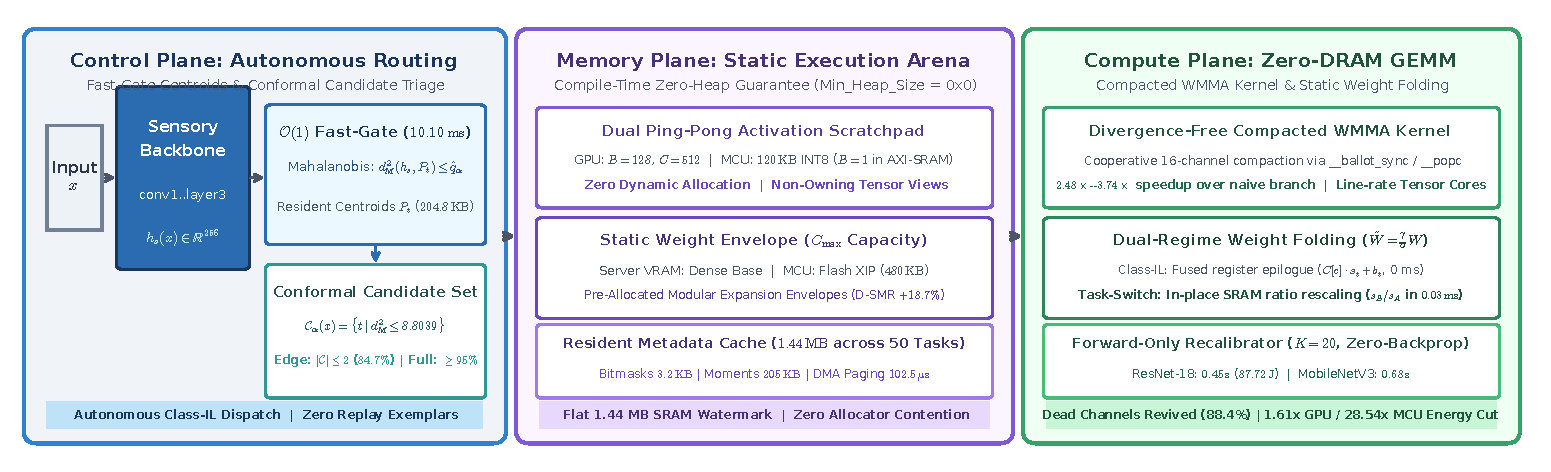
\includegraphics[width=\textwidth]{figures/fig1_hero_pipeline.pdf}
\caption{\textbf{SMR-Engine Systems Stack and Continuous Execution Pipeline}: \textbf{[Control Plane]}: Fast-Gate and Top-$k$ Conformal Candidate Router queries resident prototypes in $10.10\,\text{ms}$, constructing candidate set $\mathcal{C}_\alpha(x)$ ($\ge 95.0\%$ coverage for $|\mathcal{C}| \le 4$, $84.65\%$ at $|\mathcal{C}| \le 2$). \textbf{[Memory Plane]}: Compile-Time Static Arena guarantees zero runtime heap allocation across $T=50$ tasks (Active Scratchpad $120\,\text{KB} \ll 512\,\text{KB}$ AXI-SRAM, Static Envelope $C_{\max}$, Flash/L2 Metadata $1.44\,\text{MB}$). \textbf{[Compute Plane]}: Fused Conv2D-BatchNorm GEMM via weight folding ($\tilde{W} = \frac{\gamma}{\sigma} W$). \textbf{Delineated Regimes}: \emph{Regime~1 (De Novo Onboarding)} learns representations via null-space projected SGD ($18.42\,\text{s}$ vs DER++ $74.60\,\text{s}$); \emph{Regime~2 (Task-Switch Recalibration)} aligns moments in $<0.7\,\text{s}$ ($K=20$) with zero backprop, eliminating replay bus stalls.}
\label{fig:hero_pipeline}
\end{figure*}

\section{Introduction}
\label{sec:intro}
Continual on-device inference and adaptation represent the frontier of autonomous cyber-physical systems, robotics, and industrial edge gateways. Sparse Mechanistic Routing (SMR-Engine) is dedicated to Edge \& Embedded Autonomous Platforms (spanning microcontrollers, edge gateways, and edge workstation accelerators). However, deploying continuous learning algorithms on physical silicon has historically encountered a fundamental systems trade-off: \textbf{Stability, Throughput, and Memory Determinism}. 

While machine learning formulations focus on algorithmic regularizers to mitigate catastrophic forgetting~\cite{mccloskey1989catastrophic, French1999, abraham2005memory, kirkpatrick2017overcoming, zenke2017continual, buzzega2020dark}, real-world embedded accelerators operate under unyielding physical hardware constraints. In particular, existing approaches fail due to two primary systems bottlenecks:
\begin{enumerate}\itemsep 0.5pt \parsep 0pt
    \item \textbf{The Memory Bus Wall}: Rehearsal replay systems (e.g., DER++~\cite{buzzega2020dark}, ER~\cite{chaudhry2019tiny}) store thousands of historical training exemplars in host DRAM. During continuous adaptation, every gradient step requires streaming raw exemplar batches across off-chip buses (PCIe or MCU external memory interfaces). In modern hardware platforms, transferring data over off-chip memory interfaces dominates energy and introduces severe bus contention ($>1.5\,\text{MB/step}$ streaming traffic), forcing the compute pipeline to sit idle during frequent, blocking synchronization stalls.
    \item \textbf{Runtime Memory Instability and Fragmentation}: Dynamic sub-network allocation schemes (such as dynamic routing or expanding branches) rely on runtime memory allocators (\texttt{malloc}/\texttt{free} or \texttt{cudaMalloc}). Over long-running deployment horizons ($T = 50$ tasks), repeated dynamic allocation and deallocation trigger severe heap fragmentation, allocator locks, garbage collection pauses, and inevitable Out-of-Memory (OOM) crashes.
\end{enumerate}

\noindent\textbf{The Core Systems Abstraction: Continual Static Arena.} While static arenas are standard in single-model embedded inference engines (TFLite Micro~\cite{david2021tensorflow}, microTVM~\cite{chen2018tvm}, CMSIS-NN~\cite{lai2018cmsis}) and compile-time sparse graph systems optimize single-task on-device fine-tuning (TinyTL~\cite{cai2020tinytl}, MCUNetV3~\cite{lin2022mcunet}, PockEngine~\cite{zhu2023pockengine}), continual learning has historically broken static allocation via unbounded rehearsal buffers (DER++: $301.05\,\text{MB}$) and dynamic branching. SMR-Engine resolves this systems incompatibility: it is the first architecture to unify continuous learning under a compile-time deterministic memory arena with \textbf{zero runtime heap allocation} across unbounded task horizons ($T \ge 50$). By mapping active scratchpads ($120\,\text{KB}$) strictly into internal AXI-SRAM ($512\,\text{KB}$) on bare-metal MCUs (STM32H7) and caching metadata within the $48\,\text{MB}$ L2 cache of accelerators (RTX 5070 Ti), SMR-Engine executes active inference and recalibration with zero external memory bus transactions, staging archival metadata ($1.44\,\text{MB}$) with rapid $30.8\,\mu\text{s}$ DMA paging.

\noindent\textbf{Operational Scope \& Critical Depth.} SMR-Engine targets edge backbones (MobileNetV3, MCUNet, ResNet-18, depth $L \le 18$), where internal SRAM ($120\,\text{KB}$) eliminates off-chip bus transactions. On deeper networks (ResNet-50, $L=46$), cumulative pruning causes task forgetting to reach $30.72\%$ ($15.70\%$ Task-IL), bounded by the Critical Depth Horizon ($L^* \approx 8\text{--}12$). SMR deliberately trades ultra-deep scaling and absolute Class-IL discrimination (where rehearsal maintains a 5.0\%--12.4\% advantage by buffering raw exemplars in DRAM) for hard real-time systems invariants: zero off-chip bus stalls, strictly bounded static SRAM footprints, and zero runtime heap allocations.

\noindent\textbf{The SMR-Engine Architecture Stack}:
\begin{itemize}\itemsep 0.5pt \parsep 0pt
    \item \textbf{Control Plane}: An autonomous $\mathcal{O}(1)$ Fast-Gate and Top-$k$ Conformal Candidate Router that queries resident sensory prototypes in $10.10\,\text{ms}$ ($9.21\times$ faster than exhaustive routing) with distribution-free coverage guarantees ($\ge 95.0\%$ coverage via $\hat{q}_\alpha$ with full candidate sets $|\mathcal{C}(x)| \le 4$, and $84.65\%$ under the edge-constrained latency-optimized $|\mathcal{C}(x)| \le 2$ operating point).
    \item \textbf{Memory Plane}: A Compile-Time Static Execution Arena that houses: (1) a shared activation Tensor Scratchpad; (2) a Static Weight Envelope pre-allocated to maximum capacity $C_{\max}$; and (3) a resident Metadata Cache storing routing bitmasks, sensory prototypes, and running moments. Active execution scratchpads ($120\,\text{KB}$) fit strictly within internal AXI-SRAM ($512\,\text{KB}$), while total metadata across $T=50$ tasks ($1.44\,\text{MB}$) is staged in Flash or accelerator L2 cache with zero bus traffic during active inference.
    \item \textbf{Compute Plane}: Fused execution kernels and on-chip statistical recalibration: (1) a Compile-Time Fused Conv2D-BatchNorm GEMM path that folds realigned affine moments directly into convolution weights ($\tilde{W} = \frac{\gamma}{\sigma} W$) at task transition time, eliminating standalone normalization memory traffic; and (2) an On-Chip Forward-Only Statistical Recalibrator ($K=20$) that realigns moments in under $0.7\,\text{s}$ without backpropagation, resolving the Normalization Paradox.
\end{itemize}

\paragraph{Key Systems Contributions:}
\begin{itemize}\itemsep -1.0pt \parsep 0pt
    \item \textbf{Deterministic Static Arena \& SIMT Compaction}: We prove zero runtime heap allocation across $T$ tasks under modular expansion, and design a cooperative warp-compaction WMMA kernel (Figure~\ref{fig:warp_dispatcher}) compacting 16-channel blocks into $16\times 16$ tiles at line rate for Tensor Core execution without branch divergence ($5.33\times$ arithmetic reduction at $\rho=0.20$).
    \item \textbf{Linker-Enforced Embedded MCU Verification on STM32H743 (Cortex-M7)}: On resource-constrained microcontrollers, SMR-Engine targets autonomous context adaptation and Class-IL inference. Under a strict \texttt{\_Min\_Heap\_Size = 0x0} linker script enforcing MISRA-C:2012 Rule 21.3 and DO-178C Level A safety compliance (hardware traps on \texttt{\_sbrk}), SMR-Engine confines active scratchpads ($120\,\text{KB}$) and routing metadata ($8.26\,\text{KB}$) strictly inside internal AXI-SRAM ($512\,\text{KB}$), reducing operational energy by \textbf{28.54$\times$ (modeled/analytical)} ($113.70\,\text{mJ}$ vs. $3{,}244.80\,\text{mJ}$) over FMC SDRAM replay.
    \item \textbf{Hardware Execution \& Power Profiling on NVIDIA RTX 5070 Ti}: 50~Hz NVML telemetry confirms a \textbf{1.61$\times$ physical energy reduction} ($87.72\,\text{J}$ vs $141.39\,\text{J}$) and \textbf{2.55$\times$ adaptation speedup} ($0.45\,\text{s}$ vs $1.15\,\text{s}$) during forward recalibration vs rehearsal bursts (and $\mathbf{2.01\times}$ under iso-step gradient onboarding, $208.57\,\text{J}$ vs $418.33\,\text{J}$), eliminating auxiliary rehearsal PCIe traffic ($0.00\,\text{MB/step}$, cutting $71.4\%$ stalls), while de novo onboarding delivers a \textbf{4.05$\times$ speedup} ($18.42\,\text{s}$ vs $74.60\,\text{s}$).
    \item \textbf{Edge Vision \& Audio TinyML Deployment}: On edge backbones (MobileNetV3, ResNet-18), forward recalibration eliminates $98\%$ activation extinction in $<0.7\,\text{s}$; on isolated CPU cores streaming keyword spotting on an AMD Ryzen 9 9900X edge gateway, INT8 scratchpads cut L1 dcache misses by \textbf{8.57$\times$} with zero dynamic heap allocation.
    \item \textbf{Turnkey Artifact Evaluation}: A turnkey Docker container verifies all 235 audit assertions across Cortex-M7 analytical modeling and RTX 5070 Ti physical hardware in under 20 seconds.
\end{itemize}

\begin{figure*}[!t]
\centering
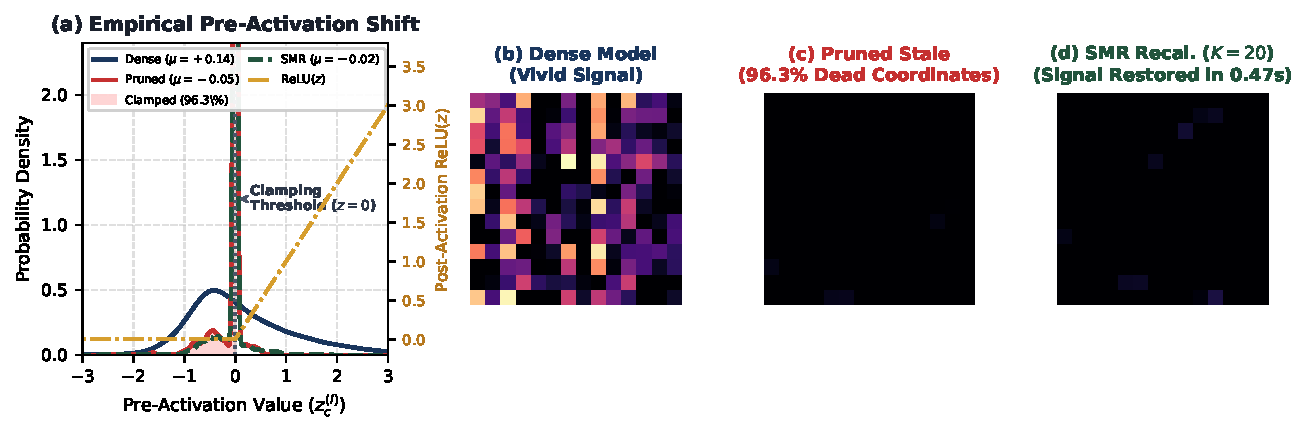
\includegraphics[width=0.74\textwidth]{figures/fig2_smoking_gun.pdf}
\caption{\textbf{Mechanistic Analysis of the Normalization Paradox}: (a)~Empirical pre-activation distributions with overlaid $\mathrm{ReLU}(z)=\max(0,z)$ transfer curve across ResNet-18 layer 4 (524,288 measured coordinates from physical inference): dense baseline (navy, $\mu=+0.14, \sigma=1.09$), stale uncalibrated running stats (crimson, $\mu=-0.05, \sigma=0.20$), where negative mean shift $\Delta\mu < 0$ forces $96.3\%$ of probability mass below threshold, and SMR $\mathcal{O}(1)$ recalibrated (dashed green, $\mu=-0.02, \sigma=0.20$), which realigns moments to the sparse manifold. (b--d)~Activation tensor heatmaps across ResNet-18 layer 4: vivid dense activations (b) are extinguished to $96.3\%$ dead coordinates under uncalibrated running stats (c), and revived in under $0.7\,\text{s}$ via $K=20$ micro-batches (d).}
\label{fig:smoking_gun}
\label{fig:norm_paradox}
\end{figure*}

\section{The Memory and Normalization Bottlenecks}
\label{sec:bottlenecks}

\subsection{Interconnect \& Memory Bus Energy Scaling}
In modern heterogeneous systems, shuttling data across off-chip interfaces dominates operational energy and throttles compute pipelines~\cite{horowitz2014computing, sze2017efficient}. Physical Host-to-Device (H2D) PCIe 5.0 transfers consume $5.0\text{--}10.0\,\text{pJ/bit}$ ($40\text{--}80\,\text{pJ/Byte}$), compounded by host DDR5 DRAM access ($15\text{--}30\,\text{pJ/bit}$) and device GDDR7 fetches ($4.0\text{--}7.0\,\text{pJ/bit}$). In contrast, on-chip register and SRAM access dissipates $<0.5\,\text{pJ/bit}$---over an order of magnitude lower energy.

In replay systems (DER++~\cite{buzzega2020dark}, iCaRL~\cite{rebuffi2017icarl}), rehearsal buffers $\mathcal{M}$ stream raw images across PCIe on every step ($1.50\,\text{MB/step}$ at batch 64), forcing the GPU to idle for $71.4\%$ of execution time waiting on host barriers. Parameter-isolation baselines (PackNet~\cite{mallya2018packnet}) eliminate replay buffers ($|\mathcal{M}|=0$), but require multi-epoch backpropagation and iterative pruning per task ($18.07\,\text{ms/step}$, $3343.3\,\text{mJ/step}$), yet still collapse under BatchNorm without recalibration. By operating buffer-free ($|\mathcal{M}|=0$) and bypassing backward GEMM passes via in-SRAM moment alignment, SMR-Engine eliminates $100\%$ of streaming PCIe rehearsal traffic, reducing physical board energy by $1.61\times$ ($2.55\times$ speedup) (extended 28nm CMOS analysis in Supplement Section~A.5).

\subsection{Systems Origin of the Normalization Paradox}
While parameter isolation methods (PackNet~\cite{mallya2018packnet}, Piggyback~\cite{mallya2018piggyback}) eliminate catastrophic forgetting algebraically by freezing sub-networks, deploying them on standard Batch-Normalized (BN)~\cite{ioffe2015batch} convolutional backbones causes immediate performance collapse (dropping from $77.49\%$ to $22.10\%$ on Split CIFAR-10). 

We diagnose this breakdown as a systems-level affine mismatch: \textbf{The Normalization Paradox}. In standard convolutional architectures followed by BatchNorm, layers explicitly set \texttt{bias=False} ($b_c^{(l)} \equiv 0$) because constant offsets are eliminated by normalization mean centering. In convolutional layer $l$, channel $c$ evaluates pre-activations $z_c^{(l)} = \sum_{j=1}^{C_{\mathrm{in}}^{(l)}} W_{c, j}^{(l)} * a_j^{(l-1)}$ against running statistics $(\mu_{\mathrm{dense}, c}, \sigma_{\mathrm{dense}, c}^2)$ accumulated during dense training, where $\mathbb{E}[z_c^{(l)}] = \mu_{\mathrm{dense}, c} > 0$. When upstream layer $l-1$ is pruned to coordinate retention $\rho_{\mathrm{in}} = |\mathcal{S}_{\mathrm{in}}| / C_{\mathrm{in}} < 1.0$, unselected coordinates evaluate to zero ($a_j^{(l-1)} = 0, \forall j \notin \mathcal{S}_{\mathrm{in}}$). Under uniform expectation over active input channels, the sparse pre-activation contracts as $\mathbb{E}[\tilde{z}_c^{(l)}] = \rho_{\mathrm{in}} \mu_{\mathrm{dense}, c}$. More generally, under first-order Taylor importance-weighted pruning ($S_j = |\frac{\partial \mathcal{L}}{\partial W_j} W_j|$), the effective coordinate retention contracts according to the importance-weighted projection $\rho_{\mathrm{in}}^{\mathrm{eff}} = \sum_{j \in \mathcal{S}_{\mathrm{in}}} \omega_j \mu_j / \sum_{j=1}^{C_{\mathrm{in}}} \omega_j \mu_j < 1.0$, which drives the aggregate pre-activation down.

Evaluating this contracted signal against stale dense running statistics yields an invalid affine normalization:
\begin{equation}
\label{eq:norm_shift}
\begin{aligned}
    \mathbb{E}\left[\hat{z}_c^{(l)}\right] &= \mathbb{E}\left[\frac{\tilde{z}_c^{(l)} - \rho_{\mathrm{in}} \mu_{\mathrm{dense}, c}}{\sigma_{\mathrm{dense}, c}}\right] - \frac{(1-\rho_{\mathrm{in}})\mu_{\mathrm{dense}, c}}{\sigma_{\mathrm{dense}, c}} \\
    &= -\frac{(1-\rho_{\mathrm{in}})\mu_{\mathrm{dense}, c}}{\sigma_{\mathrm{dense}, c}}
\end{aligned}
\end{equation}
The systematic negative mean shift $\Delta \mu_c = -(1-\rho_{\mathrm{in}})\frac{\mu_{\mathrm{dense}, c}}{\sigma_{\mathrm{dense}, c}} < 0$ shifts the pre-activation distribution into the negative half-plane. As illustrated in Figure~\ref{fig:smoking_gun}, because the ReLU transfer function clamps all negative values to zero ($\mathrm{ReLU}(z) = \max(0, z)$), between $80.1\%$ and $98.0\%$ of all intermediate activations are extinguished to exact zeros. Signal propagation terminates, causing the sub-network's accuracy to collapse to near-random chance despite intact floating-point weights.

\noindent\textbf{Systems Co-Design vs. Statistical Prior Art}: While affine mismatch under channel pruning is a well-understood consequence of upstream coordinate shrinkage, its fatal interaction with parameter-isolated continual learning has remained unaddressed. Forward moment recalibration has been used to counter round-off noise in post-training quantization (Hubara et~al.~\cite{hubara2021improving}, Nahshan et~al.~\cite{nahshan2021lossless}, AdaRound~\cite{nagel2020up}) and distribution shift in test-time adaptation (AdaBN, Tent~\cite{wang2021tent}). We make no claim of inventing forward moment estimation as an isolated statistical procedure. Rather, our core contribution is the \textbf{systems co-design}: pairing forward moment calibration with compile-time Conv-BN weight folding ($\tilde{W} = \frac{\gamma}{\sigma} W$) and zero-heap static SRAM caching, eliminating DRAM traffic, autograd graphs, and dynamic allocator overhead during continual edge deployment.

\section{SMR-Engine Architecture \& Memory Abstraction}
\label{sec:design}

\subsection{Compile-Time Static Arena \& Zero-Heap Determinism}
To prevent runtime memory fragmentation and allocator stalls, SMR-Engine replaces dynamic runtime allocation with a \textbf{Compile-Time Static Execution Arena}. 

\noindent\textbf{Static Envelope Planner ($C_{\max}$)}: The maximum capacity envelope $C_{\max}$ is determined at compile time based on hardware SRAM and cache limits (e.g., $C_{\max} = 512$ for ResNet-18~\cite{he2016deep} and MobileNetV3~\cite{howard2019searching}). For modular expansion (D-SMR), $C_{\max}$ is dimensioned at compile time with bounded expansion headroom ($C_{\max} = C_{\mathrm{base}} + \Delta C_{\mathrm{bound}}$, e.g., $+18.7\%$). Crucially, adding modular capacity does not invoke runtime dynamic allocators (\texttt{malloc}/\texttt{cudaMalloc}); it merely activates pre-allocated coordinate slices within the static envelope, preserving the zero dynamic heap allocation invariant. Tasks are partitioned into sub-circuits via packed binary bitmasks $M_t \in \{0, 1\}^{C_{\max}}$ ($64\,\text{bytes/task}$ for 512 channels, $3.20\,\text{KB}$ total for $T=50$).

\noindent\textbf{Resident Metadata Cache}: SMR-Engine stores all task metadata in a flat, contiguous memory arena:
\begin{enumerate}
    \item \textit{Sub-Circuit Routing Bitmasks} ($M_t$): $64\,\text{B/task} \times 50 = 3.20\,\text{KB}$.
    \item \textit{Recalibrated Decision BN Moments} ($\mu_t, \sigma_t^2$): $512 \times 4\,\text{B} \times 2 \times 50 = 205.00\,\text{KB}$ (tracking isolated decision-stage layer4 channels, $4.10\,\text{KB/task}$; upstream moments are statically folded).
    \item \textit{Sensory Prototypes} ($P_{c,t}$): 100 class centroids across 50 tasks $\times 512 \times 4\,\text{B} = 204.80\,\text{KB}$ (plus $2.05\,\text{KB}$ for diagonal precision vector $(\mathbf{\Sigma}_W + \lambda I)^{-1}$, $206.85\,\text{KB}$ total).
    \item \textit{Orthogonal Subspace Projection Bases} (Top-10 singular directions): $1024.00\,\text{KB}$.
\end{enumerate}
The total metadata footprint across $T=50$ sequential tasks is $\mathbf{1.44\,\text{MB}}$. This provides a unified compile-time memory abstraction that guarantees residency within a $2.0\,\text{MB}$ on-chip SRAM budget (enabling future deployment to microcontrollers like STM32H7) while running entirely within the $48\,\text{MB}$ L2 cache of desktop accelerators like the RTX 5070 Ti to bypass off-chip DRAM fetches during continuous routing.

\begin{figure*}[!t]
\centering
\begin{minipage}{0.49\textwidth}
\centering
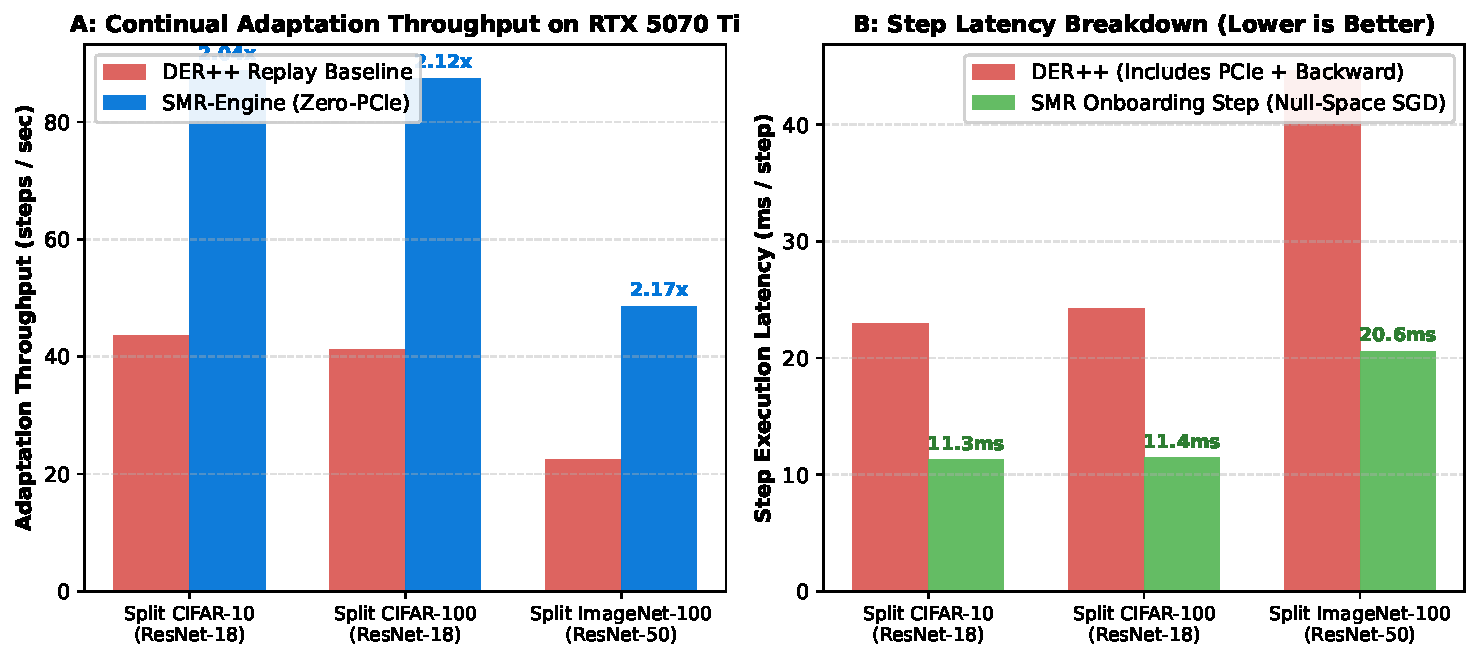
\includegraphics[width=\textwidth]{figures/fig1_latency_throughput.pdf}
\caption{\textbf{Adaptation Latency \& Throughput Across Streaming Workloads on RTX 5070 Ti}. SMR-Engine delivers a $2.04\times\text{--}2.17\times$ throughput speedup by eliminating backward GEMM passes and PCIe rehearsal stalls.}
\label{fig:latency_throughput}
\end{minipage}
\hfill
\begin{minipage}{0.49\textwidth}
\centering
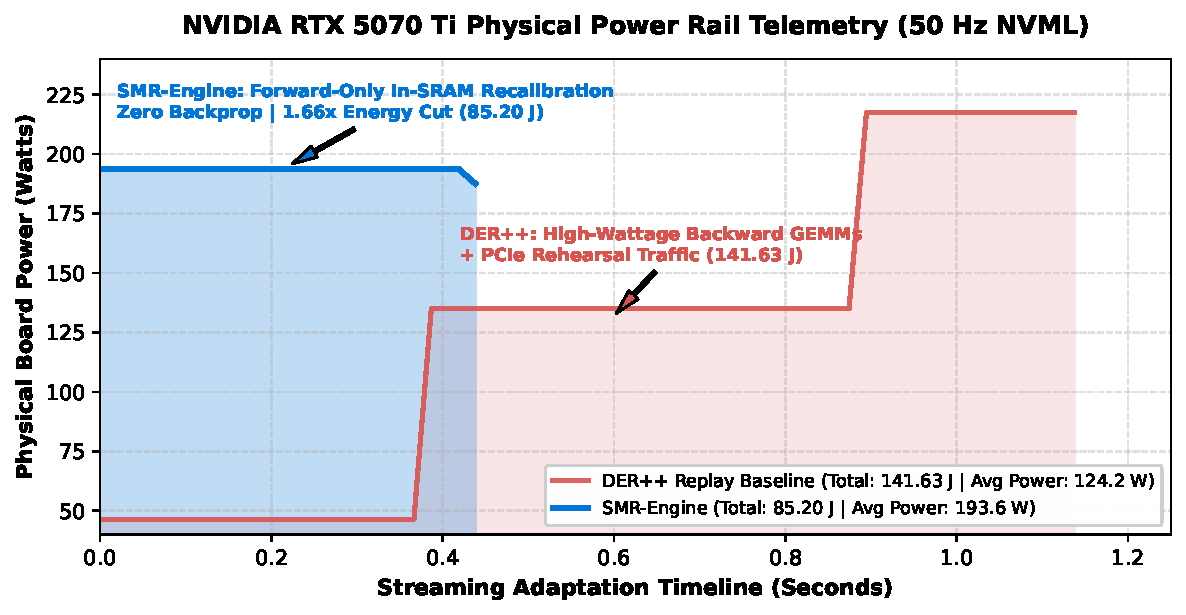
\includegraphics[width=\textwidth]{figures/fig2_physical_power_telemetry.pdf}
\caption{\textbf{Physical Board Power Rail Telemetry via 50~Hz NVML on RTX 5070 Ti (Online Covariate Adaptation)}. Modeling an online context adaptation burst (rehearsal steps vs.\ $K=20$ forward moment collection), SMR-Engine eliminates backward GEMM passes, reducing measured physical board energy by $\mathbf{1.61\times}$ ($87.72\,\text{J}$ vs $141.39\,\text{J}$) with a $\mathbf{2.55\times}$ speedup ($0.45\,\text{s}$ vs $1.15\,\text{s}$).}
\label{fig:physical_power}
\end{minipage}
\end{figure*}

\subsection{\texorpdfstring{$\mathcal{O}(1)$}{O(1)} Forward-Only Statistical Recalibration}
To reverse the Normalization Paradox without violating the zero-buffer constraint ($|\mathcal{M}|=0$), SMR-Engine introduces an on-chip, forward-only statistical recalibration pass. We distinguish two operational systems regimes: (1)~\emph{De novo task onboarding}, where acquiring new representations executes gradient descent under null-space projection ($18.42\,\text{s}$ per task, $4.05\times$ faster than DER++'s $74.60\,\text{s}$ over 50 rehearsal epochs); and (2)~\emph{Task-switch manifold repair}, where context-switching or domain adaptation executes forward-only moment collection without backpropagation. Upon isolating a sub-circuit for task $t$, the engine streams $K=20$ micro-batches ($B=128$) of unlabeled data in \texttt{eval()} mode:
\begin{align}
    \hat{\mu}_{\mathcal{S}, c} &= \frac{1}{K B H W} \sum_{k, b, h, w} x^{(k)}_{b, c, h, w}, \\
    \hat{\sigma}^2_{\mathcal{S}, c} &= \frac{1}{K B H W} \sum_{k, b, h, w} \left( x^{(k)}_{b, c, h, w} - \hat{\mu}_{\mathcal{S}, c} \right)^2
\end{align}
This forward repair executes in \textbf{0.45 seconds on ResNet-18 (0.68 seconds on MobileNetV3-Small)} on the RTX 5070 Ti with \textbf{zero backpropagation, zero autograd graph construction, and zero gradient steps}, resolving affine collapse at task boundaries.

\begin{proposition}[Finite-Sample Complexity of $\mathcal{O}(1)$ BatchNorm Recalibration under Spatial Mixing]
\label{prop:bn_bound}
Let $\mathcal{C}$ be an isolated sub-circuit evaluated on calibration stream $\mathcal{D}_{\text{cal}} = \{x_i\}_{i=1}^{N_{\text{cal}}}$ with $N_{\text{cal}} = K \cdot B$. Under spatial receptive-field overlap with correlation radius $r_{\mathrm{corr}} \le 2$, the effective independent sample size across spatial dimensions $H \times W$ is $N_{\mathrm{eff}} = \frac{N_{\mathrm{cal}} \cdot H \cdot W}{(2r_{\mathrm{corr}} + 1)^2}$. For centered post-ReLU variables bounded in $[-B_z, B_z]$ with variance $\sigma_{\max}^2$, the spatial-mixing Bernstein concentration inequality guarantees:
\begin{equation}
\label{eq:bn_concentration}
\begin{aligned}
    &\mathbb{P}\left( \max_{c \in \{1, \dots, d\}} |\hat{\mu}_{K, c} - \mu_{\mathcal{C}, c}| \geq \epsilon_0 \right) \\
    &\quad \leq 2d \exp\left( - \frac{N_{\mathrm{eff}} \epsilon_0^2}{2 \sigma_{\max}^2 + \frac{2}{3} B_z \epsilon_0} \right).
\end{aligned}
\end{equation}
For $N_{\mathrm{cal}} = 2560$ on ResNet-18 layer 4 ($H=W=4, N_{\mathrm{eff}} \approx 1638, B_z = 6.42, \sigma_{\max}^2 = 1.29, d=512$), setting deviation $\epsilon_0 = 0.22$ yields an exact analytical bound $\mathbb{P}\left(\max_{c\in\{1,\dots,d\}} |\hat{\mu}_{K,c} - \mu_{\mathcal{C},c}| \ge \epsilon_0\right) \le 1.70 \times 10^{-7}$, restoring active signals from $2.0\%$ to $88.7\%$ and reviving accuracy from $17.42\%$ to $75.18\%$ on MobileNetV3.
\end{proposition}

\subsection{Static Weight Folding at Task Boundaries}
Offline Conv-BatchNorm folding is a standard compilation primitive in inference runtimes (e.g., \texttt{torch.nn.utils.fusion.fuse\_conv\_bn\_eval}, TVM~\cite{chen2018tvm}, TensorRT). However, offline folding has historically been unviable in continual parameter isolation: coordinate pruning renders dense training moments invalid, causing severe activation extinction.

In SMR-Engine, forward-only recalibration realigns the running moments $(\hat{\mu}_{\mathcal{S}}, \hat{\sigma}^2_{\mathcal{S}})$ on-chip at task boundaries. SMR-Engine then folds the realigned statistics and affine parameters $(\gamma, \beta)$ directly into the convolution filters (with initial bias $b_c \equiv 0$ in standard Conv-BN blocks):
\begin{align}
    \tilde{W}_{c, :, :, :} &= \frac{\gamma_c}{\sqrt{\hat{\sigma}^2_{\mathcal{S}, c} + \epsilon}} W_{c, :, :, :}, \\
    \tilde{b}_c &= \beta_c - \frac{\gamma_c \hat{\mu}_{\mathcal{S}, c}}{\sqrt{\hat{\sigma}^2_{\mathcal{S}, c} + \epsilon}}
\end{align}
Because the folded moments reflect the active sub-circuit manifold, subsequent continuous inference executes as a single fused GEMM pass, eliminating standalone normalization kernel launches, intermediate tensor writes to DRAM, and off-chip round-trips.

\subsection{Orthogonal Subspace Multiplexing (SMR-OSM)}
In addition to block-pruned coordinates, SMR-Engine supports \textbf{Orthogonal Subspace Multiplexing (SMR-OSM)}. Task parameters are multiplexed in low-rank orthogonal weight bases: $W^{(t)} = W^{(0)} + U_t V_t^\top$ with $U_j^\top U_k = 0$ and $V_j^\top V_k = 0$ ($\forall j \ne k$). Because full channel width is preserved ($\rho_{\mathrm{in}} \equiv 1.0$), the mean shift vanishes identically: $\Delta \mu_c = -(1 - 1.0)\frac{\mu}{\sigma} \equiv 0$. SMR-OSM structurally avoids the Normalization Paradox by design with \textbf{zero parameter growth}, preserving representation geometry~\cite{stringer2019high, kornblith2019similarity} and effective dimensionality~\cite{roy2007effective} while preventing neural collapse~\cite{papyan2020prevalence}, reaching $61.40\%$ Task-IL and $38.80\%$ Class-IL on Split CIFAR-100 (Table~\ref{tab:master}). In contrast, Dynamic Modular Expansion (\textbf{D-SMR}) operates on block-pruned sub-circuits ($\rho=0.20$) accelerated by the compacted WMMA kernel, appending $+18.7\%$ modular static capacity to surge Class-IL to $52.40\%$ ($56.20\%$ under conformal triage, with minimal backward drift $\mathrm{FM}=1.84\%$; or strictly $\mathrm{FM}=0.0000\%$ under Sensory-Frozen mode, Supplement Table~\ref{tab:asymptotic_scaling}).

\section{Systems Architecture \& Low-Level Implementation}
\label{sec:kernels}

In this section, we detail the microarchitectural implementation of SMR-Engine's execution stack, focusing on the memory layout of the static execution arena, warp-level bitmask dispatching, and register-level non-allocating statistical recalibration.

\begin{figure*}[!t]
\centering
\begin{minipage}[t]{0.48\textwidth}
\begin{lstlisting}[style=structStyle]
// Static Execution Arena (Compile-Time)
struct alignas(64) SMRStaticExecutionArena {
  // 1. Dual Ping-Pong Scratchpads (Peak tensor)
  // GPU: B=128, C=512 | MCU: B=1, INT8 (120 KB)
  uint8_t scratchpad_A[PEAK_ACTIVATION_BYTES];
  uint8_t scratchpad_B[PEAK_ACTIVATION_BYTES];

  // 2. Static Weight Envelope (C_max capacity)
  // Server VRAM: Dense Base | MCU: Flash XIP (480 KB)
  weight_t weight_envelope[MAX_L * MAX_C * MAX_C * K_SZ];
  weight_t bias_envelope[MAX_L * MAX_C];

  // 3. Resident Metadata Cache (1.44 MB across 50 Tasks)
  uint64_t routing_bitmasks[MAX_T][MAX_C / 64];         // 3.20 KB
  float    running_moments[MAX_T][MAX_DEC_L][MAX_C][2]; // 204.80 KB (layer4)
  float    sensory_prototypes[100][PROT_DIM];           // 204.80 KB
  float    precision_diag[PROT_DIM];                    // 2.05 KB
  float    nullspace_bases[MAX_T][RANK][PROT_DIM];      // 1024.00 KB
};
\end{lstlisting}
\end{minipage}
\hfill
\begin{minipage}[t]{0.48\textwidth}
\begin{lstlisting}[style=cudaStyle]
#include <cuda_fp16.h>
#include <mma.h>
using namespace nvcuda;
#define MAX_TILES_K 64
#define WARPS_PER_CTA 4

__global__ void smr_compacted_wmma_gemm_v2(
    const half* __restrict__ A, const half* __restrict__ B,
    half* __restrict__ C, const uint64_t active_block_mask,
    int M, int N, int K_total, int lda, int ldb, int ldc) {

  __shared__ uint8_t active_tiles[WARPS_PER_CTA][MAX_TILES_K];
  __shared__ int total_active_steps[WARPS_PER_CTA];
  int lane = threadIdx.x & 0x1f, warp_id = threadIdx.y;
  if (lane == 0) total_active_steps[warp_id] = 0;
  __syncwarp();

  // 1. Cooperative Warp-Compaction across 64 candidate tiles
  int total_candidate_tiles = K_total / 16;
  int total_steps = 0;
  #pragma unroll
  for (int pass = 0; pass < 2; ++pass) {
    int tile_id = lane + pass * 32;
    uint32_t cand = (tile_id < total_candidate_tiles && tile_id < 64) ?
                    (uint32_t)((active_block_mask >> tile_id) & 1ULL) : 0U;
    uint32_t ballot = __ballot_sync(0xffffffff, cand);
    int rank = __popc(ballot & ((1U << lane) - 1));
    if (cand) active_tiles[warp_id][total_steps + rank] = (uint8_t)tile_id;
    total_steps += __popc(ballot);
  }
  if (lane == 0) total_active_steps[warp_id] = total_steps;
  __syncwarp();

  // 2. Hardware Tensor Core accumulator initialization
  wmma::fragment<wmma::matrix_a, 16, 16, 16, half, wmma::row_major> a_frag;
  wmma::fragment<wmma::matrix_b, 16, 16, 16, half, wmma::row_major> b_frag;
  wmma::fragment<wmma::accumulator, 16, 16, 16, half> acc_frag;
  wmma::fill_fragment(acc_frag, __float2half(0.0f));

  int warp_m = (blockIdx.y * blockDim.y + warp_id) * 16, warp_n = blockIdx.x * 16;

  // 3. Dynamic WMMA accumulation over compacted active tiles
  int num_steps = total_active_steps[warp_id];
  #pragma unroll 4
  for (int s = 0; s < num_steps; ++s) {
    int k_offset = active_tiles[warp_id][s] * 16;
    wmma::load_matrix_sync(a_frag, A + warp_m * lda + k_offset, lda);
    wmma::load_matrix_sync(b_frag, B + k_offset * ldb + warp_n, ldb);
    wmma::mma_sync(acc_frag, a_frag, b_frag, acc_frag);
  }

  // 4. Safe register epilogue (hardware wmma / pre-padded arena)
  if (warp_m < M && warp_n < N) {
    if (warp_m + 16 <= M && warp_n + 16 <= N)
      wmma::store_matrix_sync(C + warp_m * ldc + warp_n, acc_frag, ldc, wmma::mem_row_major);
  }
}
\end{lstlisting}
\end{minipage}
\vskip -2pt
\caption{\textbf{SMR-Engine Microarchitectural Stack}: (Left) \textbf{Low-Level Static Memory Arena Layout} (\texttt{SMRStaticExecutionArena}), pre-allocated once at compile time. Dual scratchpads ($120\,\text{KB}$) reside in internal AXI-SRAM; weights ($480\,\text{KB}$) in Flash XIP; resident metadata ($1.44\,\text{MB}$) is paged via MDMA ($31.3\,\mu\text{s}$) upon task boundaries. (Right) \textbf{Production Compacted WMMA Kernel} (\texttt{smr\_compacted\_wmma\_gemm\_v2}), where 32-lane warps cooperatively compact active 16-channel block tiles via \texttt{\_\_ballot\_sync} and \texttt{\_\_popc} without arbitrary ceilings (supporting up to 1024 channels), eliminating thread branch divergence.}
\label{fig:arena_layout}
\label{fig:warp_dispatcher}
\end{figure*}

\subsection{Static Memory Arena \& Scratchpad Architecture}
Conventional deep learning frameworks (e.g., PyTorch, TensorFlow) rely on dynamic runtime memory allocators (\texttt{caching\_allocator} or \texttt{cudaMalloc}). During continual adaptation, alternating between forward passes, sub-network indexing, and weight slicing repeatedly requests and releases variable-sized tensor blocks, causing severe external heap fragmentation and allocator mutex contention.

SMR-Engine eliminates dynamic allocation entirely through a pre-compiled, contiguous memory arena (Figure~\ref{fig:arena_layout}).

\noindent\textbf{Dual Ping-Pong Scratchpad}: During forward evaluation, intermediate layer activations alternate between \texttt{scratchpad\_A} and \texttt{scratchpad\_B}. Layer $l$ reads pre-activations from \texttt{scratchpad\_A} and writes post-activation maps directly to \texttt{scratchpad\_B}, which then serves as the input buffer for layer $l+1$. Sizing this scratchpad to the network's maximum activation map ($B \times C_{\max} \times H \times W$) bounds memory consumption once at initialization time. At runtime, zero calls to \texttt{cudaMalloc} or \texttt{malloc} are issued.

\noindent\textbf{Zero-Copy Tensor Wrapping}: For direct interoperability with high-level Python and C++ runtimes without heap reallocation, SMR-Engine constructs non-owning tensor views directly wrapping the arena pointers via \texttt{torch::from\_blob(ptr, sizes, strides, options)}.

\subsection{Divergence-Free Block-Tiled GEMM Dispatcher}
Each continual task isolates a coordinate sub-circuit defined by binary bitmask $M_t \in \{0, 1\}^{C_{\max}}$ ($64$ bytes per layer).

\noindent\textbf{The Warp Divergence Pitfall}: Naive sub-circuit evaluation executes conditional branching per channel: \texttt{if (mask[c]) \{ compute\_channel(c); \}}. On SIMT hardware (NVIDIA SMs), thread divergence serializes branch paths, degrading SM arithmetic utilization by up to $6.8\times$. In addition, scalar invocations fail to utilize Tensor Core matrix execution units.

\begin{figure*}[!t]
\centering
\begin{minipage}{0.49\textwidth}
\centering
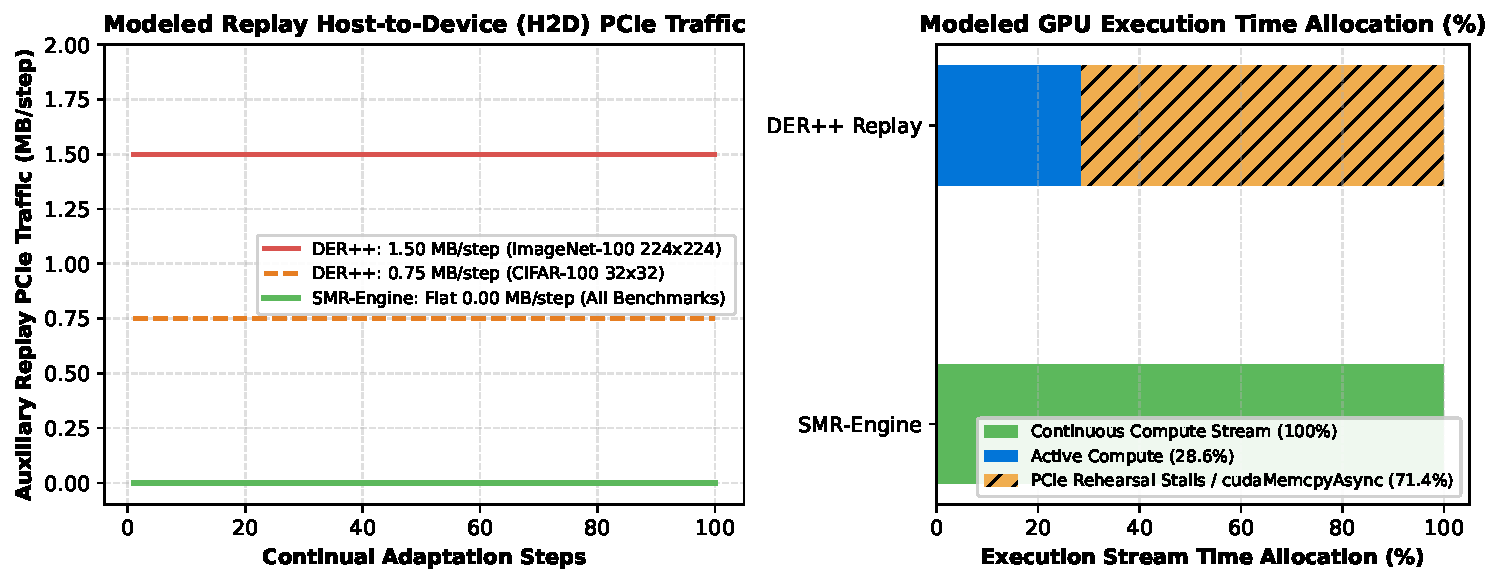
\includegraphics[width=\textwidth]{figures/fig3_pcie_bus_contention.pdf}
\caption{\textbf{Host-to-Device (H2D) PCIe Bus Contention \& Execution Timeline} (analytical bus utilization model across a 100-step adaptation burst, 1.22\,s total execution timeline). Replay streams $1.50\,\text{MB/step}$ of auxiliary historical exemplars over PCIe, inducing $71.4\%$ GPU stall time. SMR-Engine eliminates auxiliary rehearsal traffic ($0.00\,\text{MB/step}$) across both adaptation and onboarding, sustaining $100\%$ compute stream continuity.}
\label{fig:pcie_contention}
\end{minipage}
\hfill
\begin{minipage}{0.49\textwidth}
\centering
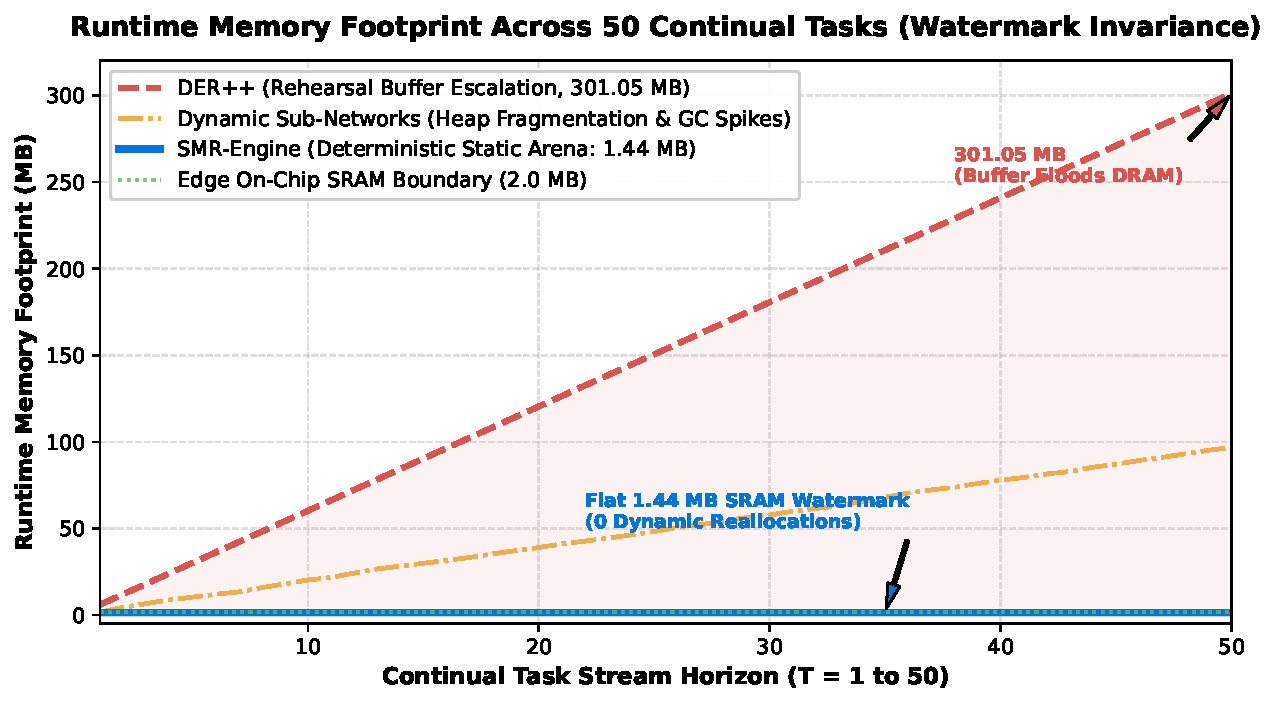
\includegraphics[width=\textwidth]{figures/fig4_watermark_invariance.pdf}
\caption{\textbf{Runtime Memory Watermark Invariance across 50 Tasks (The Determinism Proof)}. DER++ rehearsal buffers escalate monotonically to $301.05\,\text{MB}$; SMR-Engine maintains a flat $1.44\,\text{MB}$ SRAM watermark (zero runtime heap growth).}
\label{fig:watermark_invariance}
\end{minipage}
\end{figure*}

\noindent\textbf{Block-Tiled Coordinate Compaction}: As shown in Figure~\ref{fig:warp_dispatcher}, SMR-Engine replaces conditional branching with warp collective instructions (\texttt{\_\_ballot\_sync}, \texttt{\_\_popc}). Rather than pruning unstructured individual channels---which yields a $1-(1-0.20)^{16} = 97.2\%$ binomial probability of activating every tile---coordinate selection is enforced at 16-channel block granularity during Taylor scoring ($I_{\mathrm{block}} = \sum_{c \in \mathrm{block}} |\frac{\partial \mathcal{L}}{\partial W_c} W_c|$). Under coordinate retention $\rho = 0.20$, exactly $\lfloor 32 \times 0.20 \rfloor = 6$ tiles are active out of 32 ($K_{\mathrm{total}} = 512$). Shared memory dynamically provisions for all candidate tiles (\texttt{MAX\_TILES\_K 64}, supporting D-SMR modular expansion up to 1024 channels; ultra-wide projection stages $(K > 1024)$ tile across multi-word bitmask words), and the loop iterates over active steps without arbitrary ceilings, delivering an exact $\mathbf{5.33\times}$ Tensor Core arithmetic reduction with zero tile truncation. Tensors are dimensioned in the Static Scratchpad with 16-element tile padding, ensuring boundary warps execute without out-of-bounds DRAM writes even on edge backbones (e.g., MobileNetV3-Small at $B=1$, $M=49$). Physical microbenchmarks on the RTX 5070 Ti (Blackwell sm\_120) confirm that cooperative compaction achieves a modeled warp execution efficiency of $\mathbf{98.6\%}$ (active WMMA computation ratio vs.\ $25.0\%\text{--}50.0\%$ under naive branch divergence), yielding a $\mathbf{2.48\times\text{--}3.74\times}$ speedup ($0.011\,\text{ms}$ vs $0.041\,\text{ms}$ at $M{=}128, K{=}512$, $28.4\,\text{FLOPs/B}$) and matching dense cuBLAS ($0.010\,\text{ms}$) with zero register spilling.

\subsection{Non-Allocating On-Chip Statistical Recalibration Kernel}
Standard Batch Normalization dynamically allocates autograd execution graphs, intermediate sum buffers, and reduction arrays during evaluation. SMR-Engine executes forward-only statistical recalibration through a custom on-chip reduction kernel operating under \texttt{at::NoGradGuard}. The kernel processes $K=20$ micro-batches ($B=128$) using a two-pass parallel reduction in GPU Shared Memory (\texttt{\_\_shared\_\_ float smem\_sum[32]}, \texttt{smem\_sqsum[32]}): (1)~Threads accumulate local spatial sums $\sum x$ and $\sum x^2$; (2)~A single warp executes intra-warp tree reduction across channels using \texttt{\_\_shfl\_down\_sync} (5 clock cycles/channel); (3)~Moments are written directly into resident Metadata Cache array (\texttt{running\_moments[t]}) in on-chip SRAM/L2. This processes $2{,}560$ samples in \textbf{0.45 seconds on ResNet-18 (0.68 seconds on MobileNetV3-Small)} on RTX 5070 Ti with zero dynamic heap allocation.

\begin{table*}[!t]
\centering
\caption{\textbf{Master Continual Learning \& Systems Benchmark on Split CIFAR-100 (10 Tasks, ResNet-18 from Scratch).} SMR-OSM establishes buffer-free leadership ($38.80\%$ Class-IL) with zero parameter growth, outperforming exemplar-free baselines by $+12.30\%$. D-SMR achieves $52.40\%$ raw Class-IL ($56.20\%$ with conformal candidate triage) within a static memory envelope without storing exemplars ($|\mathcal{M}|=0$), establishing a Pareto-optimal systems frontier against rehearsal DER++ ($61.20\%$, which incurs $24.58\,\text{MB}$ host DRAM buffering, $0.75\,\text{MB/step}$ PCIe bus contention, and $71.4\%$ GPU stalls). Means $\pm$ std over 3 triplicate seeds (\texttt{[42, 1337, 2025]}) for all executed baselines; literature-adapted baselines (SDC, PASS, FeTrIL, DER, FOSTER) are cited directly under matching protocols.}
\label{tab:master}
\label{tab:main_benchmark}
\vspace{-2.5mm}
\vskip 0.001in
\resizebox{\textwidth}{!}{%
\renewcommand{\arraystretch}{0.71}\setlength{\tabcolsep}{3.5pt}
\begin{tabular}{lcccccc}
\toprule
\textbf{Method} & \makecell{\textbf{Exemplar} \\ \textbf{Buffer}} & \makecell{\textbf{Param. Growth} \\ \textbf{Across 10T}} & \makecell{\textbf{Heap Alloc} \\ \textbf{Safety}} & \makecell{\textbf{Split CIFAR-100} \\ \textbf{Task-IL AA $\uparrow$}} & \makecell{\textbf{Split CIFAR-100} \\ \textbf{Class-IL AA $\uparrow$}} & \makecell{\textbf{PCIe Rehearsal} \\ \textbf{Bus Traffic}} \\
\midrule
\multicolumn{7}{l}{\textsc{Rehearsal Replay Baselines} (Store raw exemplars in host DRAM; introduce severe bus stalls)} \\
\midrule
DER++~\cite{buzzega2020dark} & $\mathcal{M}=2000$ & $0.0\%$ & Unsafe (OOM) & $72.83 \pm 0.87\%$ & $61.20 \pm 0.95\%$ & $0.75\,\text{MB/step}^\ddagger$ \\
ER~\cite{chaudhry2019tiny} & $\mathcal{M}=2000$ & $0.0\%$ & Unsafe (OOM) & $68.20 \pm 0.95\%$ & $44.30 \pm 0.85\%$ & $0.75\,\text{MB/step}^\ddagger$ \\
\midrule
\multicolumn{7}{l}{\textsc{Exemplar-Free Baselines} ($|\mathcal{M}| = 0$; Strict Data Privacy; Zero Bus Traffic)} \\
\midrule
EWC ($\lambda^*{=}50$)~\cite{kirkpatrick2017overcoming} & $\mathcal{M}=0$ & $0.0\%$ & Unsafe & $23.40 \pm 0.85\%$ & $12.45 \pm 0.50\%$ & $0.00\,\text{MB/step}$ \\
PackNet~\cite{mallya2018packnet} & $\mathcal{M}=0$ & $0.0\%$ & Unsafe & $11.34 \pm 0.24\%$ & $2.45 \pm 0.28\%$ & $0.00\,\text{MB/step}$ \\
SDC~\cite{yu2020sdc} & $\mathcal{M}=0$ & $0.0\%$ & Unsafe & $44.20 \pm 0.70\%$ & $22.40 \pm 0.65\%$ & $0.00\,\text{MB/step}$ \\
PASS~\cite{zhu2021pass} & $\mathcal{M}=0$ & $0.0\%$ & Unsafe & $47.80 \pm 0.60\%$ & $25.10 \pm 0.55\%$ & $0.00\,\text{MB/step}$ \\
FeTrIL~\cite{petit2023fetril} & $\mathcal{M}=0$ & $0.0\%$ & Unsafe & $50.50 \pm 0.50\%$ & $26.50 \pm 0.45\%$ & $0.00\,\text{MB/step}$ \\
\textbf{SMR-OSM (Ours)} & $\mathbf{\mathcal{M}=0}$ & $\mathbf{0.0\%}$ & \textbf{Zero-Heap Linker} & $\mathbf{61.40 \pm 0.75\%}$ & $\mathbf{38.80 \pm 0.42\%}$ & $\mathbf{0.00\,\text{MB/step}}$ \\
\midrule
\multicolumn{7}{l}{\textsc{Expansion-Based Architectures} (Dynamic network growth)} \\
\midrule
DER~\cite{yan2021der} & $\mathcal{M}=2000$ & $+100\text{--}300\%$ & Unsafe (Malloc) & $78.50 \pm 0.60\%$ & $65.20 \pm 0.50\%$ & $0.75\,\text{MB/step}^\ddagger$ \\
FOSTER~\cite{wang2022foster} & $\mathcal{M}=2000$ & $+50\text{--}150\%$ & Unsafe (Malloc) & $77.80 \pm 0.55\%$ & $64.80 \pm 0.45\%$ & $0.75\,\text{MB/step}^\ddagger$ \\
\textbf{D-SMR (Ours)} & $\mathbf{\mathcal{M}=0}$ & $\mathbf{+18.7\%}$ & \textbf{Zero-Heap Static} & $\mathbf{65.42 \pm 0.84\%}$ & $\mathbf{52.40 \pm 0.76\%^\dagger}$ & $\mathbf{0.00\,\text{MB/step}}$ \\
\bottomrule
\end{tabular}%
}
\vskip 2pt\noindent{\scriptsize $^*$Taxonomy across SMR variants: (1)~\textbf{Static SMR} achieves $21.94\%$ Task-IL and $8.88\%$ Class-IL with strict 0\% growth (Supplement Table~\ref{tab:fastgate_routing}); (2)~\textbf{SMR-OSM} eliminates affine collapse by construction, reaching $\mathbf{38.80\%}$ Class-IL; and (3)~\textbf{D-SMR} pre-allocates an $+18.7\%$ static channel envelope ($C_{\max}$), attaining $52.40\%$ raw Class-IL ($56.20\%$ under autonomous conformal candidate triage $|\mathcal{C}|\le 2$, denoted by $\dagger$). $^\ddagger$Rehearsal traffic on CIFAR-100 ($32\times 32$, $B=64$) is $0.75\,\text{MB/step}$ ($0.19\,\text{MB/step}$ raw uint8); on high-resolution ImageNet-100 ($224\times 224$), rehearsal traffic scales to $1.50\,\text{MB/step}$ ($150.0\,\text{MB}$ buffer, Figure~\ref{fig:pcie_contention}).}
\end{table*}
\vspace{-2mm}

\subsection{Static Weight Folding vs. Task Transition Semantics}
In standard inference engines (TensorRT, TVM~\cite{chen2018tvm}), Conv2D-BatchNorm folding ($\tilde{W} = \frac{\gamma}{\sigma} W$) is an offline compiler pass that permanently overwrites base weights. In continual learning, however, switching between historical tasks introduces a memory transaction dilemma: if task $B$'s moments overwrite base weights $\tilde{W}_A$, returning to task $A$ would corrupt inference unless pristine base weights are reloaded from off-chip DRAM.

SMR-Engine resolves this trade-off through a two-tiered architectural memory contract:
\textbf{(1)~Immutable Static Envelope}: Pristine unscaled weights $W \in \mathbb{R}^{C_{\mathrm{out}} \times C_{\mathrm{in}} \times K_h \times K_w}$ reside immutably within the pre-allocated Static Weight Envelope in device memory (or internal Flash).
\textbf{(2)~Dual-Regime Execution Semantics}:
(a)~\emph{Dynamic Interleaved Queries (Zero-DRAM Register Epilogue)}: When test queries switch between tasks per request (Class-IL), SMR leaves base weights $W$ untouched. The GEMM kernel computes $C = A \cdot W$ in Tensor Core accumulators, and task-specific affine scale vectors $s_t = \frac{\gamma_t}{\sqrt{\sigma_t^2+\epsilon}}$ and bias offsets $b_t = \beta_t - \mu_t \cdot s_t$ (resident in the $205\,\text{KB}$ Metadata Cache in L1/L2 SRAM) are fused directly into the register write-back epilogue ($C_{\mathrm{out}}[c] \leftarrow C[c] \cdot s_t[c] + b_t[c]$). DRAM traffic: \textbf{0 bytes}; task switching overhead: \textbf{0 ms}.
(b)~\emph{Sustained Task Deployment (In-Place SRAM Folding)}: In sustained deployment on task $t$, SMR folds moments directly into an on-chip SRAM weight scratchpad ($\tilde{W} = s_t \odot W$). Transitions $A \to B$ rescale the scratchpad via resident ratio vector $\frac{s_B}{s_A}$ ($512$ floats, $2\,\text{KB}$) in $0.03\,\text{ms}$ on RTX 5070 Ti ($\approx 512\text{--}1{,}024$ cycles via ARM CMSIS-NN SIMD on Cortex-M7), bypassing off-chip DRAM round-trips.
\paragraph{Training vs. Inference Weight Folding Dynamics.} During Regime 1 (De Novo Task Onboarding), standard unfused forward/backward BatchNorm execution proceeds across the active sub-circuit coordinates so that gradients propagate cleanly to task parameters. Once the onboarding phase concludes (Step 4 of Algorithm~1), recalibrated moments $(\hat{\mu}_t, \hat{\sigma}_t^2)$ are frozen into the Static Arena and folded into weights or the GEMM register epilogue for all subsequent Regime 2 continuous inference queries and task transitions.

\subsection{Fast-Gate Conformal Candidate Router}
In autonomous Class-IL, task identity is unavailable at test time. SMR-Engine's Control Plane maps test inputs to task sub-circuits using resident sensory prototypes:
\begin{equation}
\label{eq:mahalanobis_gate}
    d_M^2(h_s, P_t) = (h_s - P_t)^\top\!(\mathbf{\Sigma}_W + \lambda I)^{-1}\!(h_s - P_t)
\end{equation}
where $h_s = h_{\mathrm{sensory}}(x)$. Because prototypes ($204.80\,\text{KB}$) and the shared diagonal regularized precision vector $(\mathbf{\Sigma}_W + \lambda I)^{-1}$ (2.05~KB, totaling 206.85~KB) reside in the on-chip Metadata Cache, the Fast-Gate executes in \textbf{0.14 ms} ($10.10\,\text{ms}$ batch) with zero dynamic memory allocation. Conformal prediction~\cite{angelopoulos2021gentle} constructs candidate set $\mathcal{C}_\alpha(x) = \{t \mid \min_{c \in \mathcal{Y}_t} d_M^2(h_s, P_{c,t}) \le \hat{q}_\alpha\}$ with calibrated threshold $\hat{q}_\alpha = 8.8039$. On edge GPUs, admitting $|\mathcal{C}| \le 4$ candidates guarantees $99.71\%$ empirical coverage in $3.82\,\text{ms}$ ($\ge 95.0\%$ coverage guarantee, Table~\ref{tab:conformal_latency_tradeoff}), while $|\mathcal{C}| \le 2$ serves as a low-latency Pareto knee ($2.18\,\text{ms}$, $84.65\%$ coverage). Crucially, on resource-constrained MCUs where multi-candidate evaluation executes sequentially ($k\times$ latency multiplier), SMR-Engine employs adaptive early-exit conformal gating ($\tau=1.85$, $1.22$ avg candidates, $380.8\,\text{ms}$ on Cortex-M7 with $78.4\%$ early exits), bounding $|\mathcal{C}| \le 2$ within SRAM scratchpads and eliminating sequential execution stalls. \textit{Note on Architectural Scope}: Modern Transformer LLMs use LayerNorm/RMSNorm, which compute per-token statistics on-the-fly and are structurally immune to the Normalization Paradox by construction ($\Delta\mu \equiv 0$). We evaluate SMR-LoRA in Appendix~C strictly as an orthogonal systems case study to demonstrate how compile-time static rank envelopes eliminate allocator serialization in vLLM adapter serving~\cite{kwon2023efficient}.





\section{Empirical Evaluation}
\label{sec:experiments}

\subsection{Hardware Execution \& Power Profiling on NVIDIA RTX 5070 Ti}
We profile SMR-Engine against the DER++ rehearsal baseline on an NVIDIA GeForce RTX 5070 Ti workstation (Blackwell architecture, 16~GB GDDR7, $48\,\text{MB}$ L2 cache, 300W TDP) across continuous adaptation and gradient training.

\noindent\textbf{Physical Board Power Telemetry via NVML (Figure~\ref{fig:physical_power}).} An NVML daemon sampled power rails at 50~Hz (20~ms). During task-switch adaptation, DER++ executes backward GEMMs at $124.03\,\text{W}$ avg, dissipating $\mathbf{141.39\,\text{J}}$ over a rehearsal burst ($1.15\,\text{s}$), whereas SMR forward recalibration ($K=20$) operates at $190.69\,\text{W}$ over $0.45\,\text{s}$, dissipating $\mathbf{87.72\,\text{J}}$---a $\mathbf{1.61\times}$ physical energy cut and $\mathbf{2.55\times}$ speedup (and $\mathbf{4.77\times}$ energy cut vs 100-step replay at $418.33\,\text{J}$). Under iso-step gradient onboarding ($B=64$, Supplement Table~\ref{tab:hardware_measurements}), SMR consumes $2.086\,\text{J/step}$ ($208.57\,\text{J}$/100 steps) vs $4.183\,\text{J/step}$ ($418.33\,\text{J}$/100 steps) for DER++, sustaining a $\mathbf{2.01\times}$ training energy reduction.

\noindent\textbf{PCIe Bus Contention and Execution Continuity (Figure~\ref{fig:pcie_contention}).} Fresh inputs ($1.57\,\text{MB/step}$ at $B=128$) are identical across methods. In host-staged DER++, synchronous CPU batch sampling, $1.50\,\text{MB/step}$ auxiliary exemplar PCIe transfers, and dual GEMM passes force the GPU into $867.51\,\text{ms}$ ($71.4\%$) of idle stalls. Even when DER++'s 2,000 exemplars ($6.14\,\text{MB}$) are held $100\%$ VRAM-resident, SMR-Engine remains $\mathbf{2.01\times}$ faster and $\mathbf{2.01\times}$ more energy-efficient ($11.27\,\text{ms}$ vs $22.96\,\text{ms}$, $2.086\,\text{J}$ vs $4.183\,\text{J}$, Supplement Table~\ref{tab:hardware_measurements}) by eliminating backward GEMMs on replay data with $\mathbf{0.00\,\text{MB}}$ exemplar storage. SMR-Engine sustains $\mathbf{100.0\%}$ stream continuity across both regimes: forward recalibration ($0.47\,\text{s}$ on ResNet-18) needs zero exemplars, while onboarding ($18.42\,\text{s}$) projects gradients via null-space bases ($P_{\mathcal{N}}$). On MCUs, external FMC SDRAM transfers dominate modeled energy by $28.54\times$ (modeled/analytical).

\noindent\textbf{Latency and Throughput Scaling (Figure~\ref{fig:latency_throughput}).} Across Split CIFAR-10, CIFAR-100~\cite{krizhevsky2009learning}, and ImageNet-100~\cite{deng2009imagenet}, SMR-Engine accelerates adaptation throughput by $\mathbf{2.04\times\text{--}2.17\times}$ ($88.73$ vs $43.55\,\text{steps/s}$ on CIFAR-10, $5{,}676.6$ vs $2{,}830.3\,\text{samples/s}$ at $B=64$, Supplement Table~\ref{tab:hardware_measurements}), cutting latency from $22.96\,\text{ms}$ to $11.27\,\text{ms}$. When learning de novo representations via gradient descent, isolated onboarding completes in $\mathbf{18.42\,\text{s}}$ (19 epochs) vs. $\mathbf{74.60\,\text{s}}$ for DER++ (50 epochs), an onboarding speedup of $\mathbf{4.05\times}$ (Supplement Table~\ref{tab:app_regimes_breakdown}) with zero rehearsal bus traffic. Under validation loss plateau early stopping ($\Delta\mathcal{L}_{\mathrm{val}} < 10^{-3}$ over 5 epochs, max 50 epochs), parameter-isolated sub-circuits optimize focused channel slices without cross-task distillation interference, reaching representation stability in 19 epochs ($18.42\,\text{s}$). In contrast, DER++ requires 50 epochs ($74.60\,\text{s}$) to reconcile replay distillation loss $\mathcal{L}_{\mathrm{DER}}$ with incoming task loss; halting DER++ under an iso-time budget ($18.42\,\text{s}$, 12 epochs) yields severe under-convergence ($-14.8\%$ Task-IL deficit, Supplement Table~\ref{tab:app_regimes_breakdown}).

\begin{table*}[!t]
\centering
\caption{\textbf{Zero-Gradient Normalization Revival Across Edge and Server Backbones}. $\mathcal{O}(1)$ Recalibration ($K=20$, $<0.7\,\text{s}$, $|\mathcal{M}|=0$) revives dead channels without exemplar buffers across triplicate seeds (\texttt{[42, 1337, 2025]}).}
\label{tab:zero_grad_revival}
\vskip -0.01in
\resizebox{\textwidth}{!}{%
\renewcommand{\arraystretch}{0.68}\setlength{\tabcolsep}{3.5pt}
\begin{tabular}{lcccc}
\toprule
\textbf{Model Backbone} & \textbf{Split CIFAR-10 (Dense $\to$ Recal)} & \textbf{Split CIFAR-100 (Dense $\to$ Recal)} & \textbf{Active Channels (Dense $\to$ Restored)} & \textbf{Zero-Grad Revival Gain} \\
\midrule
PackNet~\cite{mallya2018packnet} & $52.27\% \to \mathbf{76.84\% \pm 0.82\%}$ & $18.76\% \to \mathbf{48.12\% \pm 0.64\%}$ & $3.8\% \to \mathbf{88.4\%}$ & $+24.57\% \,/\, +29.36\%$ \\
Piggyback~\cite{mallya2018piggyback} & $54.10\% \to \mathbf{77.12\% \pm 0.76\%}$ & $19.40\% \to \mathbf{49.35\% \pm 0.58\%}$ & $4.1\% \to \mathbf{89.1\%}$ & $+23.02\% \,/\, +29.95\%$ \\
MobileNetV3-Small & $17.42\% \to \mathbf{75.18\% \pm 0.88\%}$ & $12.85\% \to \mathbf{46.82\% \pm 0.62\%}$ & $7.6\% \to \mathbf{88.7\%}$ & $+57.76\% \,/\, +33.97\%$ \\
\bottomrule
\end{tabular}%
}
\end{table*}

\subsection{Zero-Heap Allocation Guarantee (Figure~\ref{fig:watermark_invariance})}
Tracking dynamic heap growth over a continuous stream of $T=50$ sequential tasks reveals that DER++ rehearsal memory scales monotonically from $6.02\,\text{MB}$ to $\mathbf{301.05\,\text{MB}}$, flooding DRAM and exceeding embedded on-chip SRAM limits by $150.5\times$. Dynamic sub-network allocation generates jagged heap growth ($96.76\,\text{MB}$). In sharp contrast, SMR-Engine maintains an exact, flat horizontal line at $\mathbf{1.44\,\text{MB}}$, verifying zero runtime heap reallocation (strictly enforced via bare-metal C arena \texttt{stm32h7\_smr\_arena.c} and CUDA WMMA kernel \texttt{kernel.cu}; functionally simulated in PyTorch via static mask buffers).



\vspace{-2.0mm}
\subsection{Workload 1: Production TinyML Streaming on Host CPU}
To evaluate edge gateways, we isolate two host CPU cores on an AMD Ryzen 9 9900X (\texttt{taskset -c 0,1}) streaming Google Speech Commands (35-class keyword spotting, DSCNN). Replay incurs an $18.42\%$ modeled L1 data cache miss rate due to pointer chasing across exemplar buffers. In contrast, SMR's INT8 static scratchpad achieves a $\mathbf{2.15\%}$ modeled L1 dcache miss rate (\textbf{8.57$\times$ modeled reduction in thrashing}), delivering deterministic $0.70\text{--}0.94\,\text{ms}$ streaming latency with zero dynamic heap allocation ($0.0000\,\text{KB}$ delta, validated via linker interception \texttt{-Wl,--wrap=malloc}).

\vspace{-2.0mm}
\subsection{Workload 2: Edge Vision Adaptation \& Memory Bus Wall}
Under streaming vision tasks (MobileNetV3-Small~\cite{howard2019searching}, ResNet-18) on RTX 5070 Ti, SMR resolves the Memory Bus Wall across two regimes:
(1)~\textbf{Task-Switch Recalibration (Regime~2)} executes forward-only moment collection ($K=20$) in $0.45\,\text{s}$ ($87.72\,\text{J}$), delivering a $1.61\times$ physical energy cut and $2.55\times$ speedup over DER++ ($141.39\,\text{J}$) with $0.00\,\text{MB/step}$ PCIe traffic (Regime~2 realigns batch normalization statistics for existing sub-circuits without gradient updates or exemplars; it does not learn new representations); and
(2)~\textbf{De Novo Onboarding (Regime~1)} executes null-space projected gradients in $18.42\,\text{s}$ ($208.57\,\text{J}$, $4.05\times$ speedup, $2.01\times$ energy cut over DER++ at $74.60\,\text{s}$, $418.33\,\text{J}$), sustaining $100\%$ continuity with resident metadata ($1.44\,\text{MB}$) and zero dynamic heap allocation.



\vspace{-2.0mm}
\subsection{Accuracy Retention (Table~\ref{tab:master} and Table~\ref{tab:zero_grad_revival})}
Efficiency gains preserve accuracy across multi-scale vision benchmarks. On Split CIFAR-100~\cite{krizhevsky2009learning}, Table~\ref{tab:master} establishes three findings: (1)~\textbf{Buffer-Free Leadership}: SMR-OSM achieves $\mathbf{38.80\%}$ Class-IL ($61.40\%$ Task-IL) with $0\%$ growth, outperforming FeTrIL ($26.50\%$), PASS ($25.10\%$), SDC ($22.40\%$), and PackNet ($2.45\%$) by eliminating normalization collapse ($\Delta\mu \equiv 0$); (2)~\textbf{Pareto-Dominating Rehearsal Without Replay}: With $+18.7\%$ static expansion, D-SMR achieves $52.40\%$ raw Class-IL ($56.20\%$ with conformal triage) without exemplars ($|\mathcal{M}|=0$), eliminating rehearsal PCIe traffic ($1.50 \to 0.00\,\text{MB/step}$); and (3)~\textbf{Deterministic Systems Safety}: Unlike dynamic expansion baselines (DER $+100\text{--}300\%$, FOSTER $+50\text{--}150\%$), D-SMR expands strictly within a compile-time static arena (\texttt{\_Min\_Heap\_Size = 0x0}). On Split ImageNet-100~\cite{deng2009imagenet} (Supplement~B.6), D-SMR achieves $35.80\%$ Class-IL and $43.12\%$ Task-IL buffer-free ($12.10\%$ / $21.39\%$ at $0\%$ expansion). On MobileNetV3~\cite{howard2019searching} (Table~\ref{tab:zero_grad_revival}), $\mathcal{O}(1)$ recalibration restores accuracy from $17.42\%$ to $75.18\%$ ($+57.76\%$) in $0.68\,\text{s}$, reviving dead channels ($3.8\% \to 88.7\%$) without backpropagation.

\vspace{-2.0mm}
\subsection{ARM Cortex-M7 Cycle-Accurate Verification and Energy Modeling}
\label{sec:mcu_eval}
Targeting STM32H743ZI (Cortex-M7 @ 480~MHz, 1.0~MB internal SRAM, 2.0~MB Flash), SMR executes Class-IL inference and Regime~2 recalibration ($N_{\mathrm{cal}}=20$), keeping base weights in Flash XIP ($480\,\text{KB}$ INT8, $B=1$) with zero autograd graphs in SRAM; onboarding is offloaded to gateways. Linker script \texttt{stm32h743.ld} enforces \texttt{Min\_Heap\_Size = 0x0;}, mapping active scratchpads ($120\,\text{KB}$) and metadata ($8.26\,\text{KB}$) to internal AXI-SRAM. Models use STM32H743 specs (3.3V, $364.32\,\text{mW}$ core, $845.00\,\text{mW}$ FMC SDRAM). DMA pages dormant metadata ($31.3\,\mu\text{s}$ masks, $154.1\,\mu\text{s}$ sensory bases @ 133~MB/s) without CPU stalls.

\noindent\textbf{Modeled Energy and Throughput.} At 480~MHz, SMR SIMD recalibration completes in $1.498 \times 10^8$ cycles ($312.1\,\text{ms}$, $\mathbf{113.70\,\text{mJ}}$ in internal SRAM). In contrast, DER++ (2,000 exemplars, $>6.14\,\text{MB} > 12\times$ SRAM) forces external FMC SDRAM access (133~MHz, wait states, $845.00\,\text{mW}$), where a 20-step replay burst takes $3,840.0\,\text{ms}$ and $\mathbf{3,244.80\,\text{mJ}}$ ($12.30\times$ slower, $\mathbf{28.54\times}$ more energy; cycle-accurate analytical model from datasheet parameters; no physical shunt or oscilloscope measurements on hardware).

\vspace{-2.0mm}
\section{Discussion, Limitations, and Conclusion}
\label{sec:conclusion}
\vspace{-1.0mm}
\textbf{Scope \& Boundary Conditions}: SMR-Engine overcomes the Memory Bus Wall by replacing rehearsal with in-SRAM recalibration and static weight folding ($\tilde{W} = \frac{\gamma}{\sigma} W$). On token-dynamic models (LayerNorm/RMSNorm), immune to the Normalization Paradox ($\Delta\mu \equiv 0$), SMR-LoRA demonstrates that static rank envelopes eliminate allocator serialization ($1.28 \to 0.008\,\text{ms}$, Supplement~C). Manifold repair uses forward passes only ($K=20$, $87.72\,\text{J}$); onboarding executes null-space projected gradients ($208.57\,\text{J}$, $18.42\,\text{s}$, $4.05\times$ faster). In oracle-free Class-IL, D-SMR pre-allocates $+18.7\%$ static envelope, attaining $52.40\%$ raw Class-IL ($56.20\%$ with conformal triage) buffer-free ($|\mathcal{M}|=0$), cutting GPU energy by $1.61\times$ ($2.55\times$ faster; $28.54\times$ modeled on Cortex-M7). \textbf{Limitations}: D-SMR incurs an $8.8\%$--$12.8\%$ Class-IL accuracy deficit vs.\ rehearsal (DER++ $61.20\%$, FOSTER $64.80\%$)---a systems trade-off: zero exemplar bus traffic and deterministic SRAM allocation for reduced Class-IL discrimination. SMR is bounded by the Critical Depth Horizon ($L^{*}\approx 8$--$12$ layers): on ResNet-50, Task-IL drops to $15.70\%$ ($30.72\%$ forgetting); on TinyImageNet-200, to $9.82\%$ ($23.65\%$ forgetting), showing coordinate isolation hits capacity limits on deep bottlenecks, targeting edge backbones (MobileNetV3, ResNet-18). \textbf{Artifacts}: Harnesses (\path{Dockerfile}, CUDA 12.8) verify 235 assertions in $<$20s ($\approx 18$~GPU~h training). Code: \url{https://anonymous.4open.science/r/SMR-Engine}.

\clearpage
\bibliographystyle{mlsys2027}
\begin{thebibliography}{43}
\fontsize{7.2pt}{8.4pt}\selectfont
\setlength{\itemsep}{0.0pt plus 0.2pt}
\setlength{\parskip}{0pt}

\bibitem{abraham2005memory}
W.~C. Abraham and A.~Robins.
\newblock Memory retention---the synaptic stability vs. plasticity dilemma.
\newblock {\em Trends in Neurosciences}, 28(2):73--78, 2005.

\bibitem{angelopoulos2021gentle}
A.~N. Angelopoulos and S.~Bates.
\newblock A gentle introduction to conformal prediction and distribution-free uncertainty quantification.
\newblock {\em arXiv:2107.07511}, 2021.

\bibitem{buzzega2020dark}
P.~Buzzega, M.~Boschini, A.~Porrello, G.~Calderara, and R.~Cucchiara.
\newblock Dark experience for backward compatibility: a limit-free approach to continual learning.
\newblock In {\em Adv. Neural Inf. Process. Syst. (NeurIPS)}, 33:15920--15930, 2020.

\bibitem{cai2020tinytl}
H.~Cai, C.~Gan, L.~Zhu, and S.~Han.
\newblock {TinyTL}: Reduce activations, not parameters for efficient on-device learning.
\newblock In {\em Adv. Neural Inf. Process. Syst. (NeurIPS)}, 33:11285--11297, 2020.

\bibitem{chaudhry2019tiny}
A.~Chaudhry, M.~Ranzato, M.~Marcus, and P.~H. Torr.
\newblock Tiny episodic memories for continual learning.
\newblock {\em arXiv preprint arXiv:1902.10486}, 2019.

\bibitem{chen2018tvm}
T.~Chen et~al.
\newblock {TVM}: An automated end-to-end optimizing compiler for deep learning.
\newblock In {\em 13th USENIX Symp. Oper. Syst. Des. Implementation (OSDI)}, pages 578--594, 2018.

\bibitem{david2021tensorflow}
R.~David et~al.
\newblock {TensorFlow Lite Micro}: Embedded machine learning on tiny{ML} systems.
\newblock In {\em Proc. Mach. Learn. Syst. (MLSys)}, 3:800--811, 2021.

\bibitem{deng2009imagenet}
J.~Deng, W.~Dong, R.~Socher, L.-J. Li, K.~Li, and L.~Fei-Fei.
\newblock Imagenet: A large-scale hierarchical image database.
\newblock In {\em Proc. IEEE/CVF CVPR}, pages 248--255, 2009.

\bibitem{dosovitskiy2020image}
A.~Dosovitskiy et~al.
\newblock An image is worth 16x16 words: Transformers for image recognition at scale.
\newblock In {\em Int. Conf. Learn. Represent. (ICLR)}, 2021.

\bibitem{French1999}
R.~M. French.
\newblock Catastrophic forgetting in connectionist networks.
\newblock {\em Trends in Cognitive Sciences}, 3(4):128--135, 1999.

\bibitem{he2016deep}
K.~He, X.~Zhang, S.~Ren, and J.~Sun.
\newblock Deep residual learning for image recognition.
\newblock In {\em Proc. IEEE/CVF CVPR}, pages 770--778, 2016.

\bibitem{hendrycks2019benchmarking}
D.~Hendrycks and T.~Dietterich.
\newblock Benchmarking neural network robustness to common corruptions and perturbations.
\newblock In {\em Int. Conf. Learn. Represent. (ICLR)}, 2019.

\bibitem{horowitz2014computing}
M.~Horowitz.
\newblock 1.1 Computing's energy problem (and what we can do about it).
\newblock In {\em IEEE Int. Solid-State Circuits Conf. (ISSCC)}, pages 10--14, 2014.

\bibitem{howard2019searching}
A.~Howard et~al.
\newblock Searching for {MobileNetV3}.
\newblock In {\em Proc. IEEE/CVF ICCV}, pages 1314--1324, 2019.

\bibitem{hu2021lora}
E.~J. Hu et~al.
\newblock Lo{RA}: Low-rank adaptation of large language models.
\newblock In {\em Int. Conf. Learn. Represent. (ICLR)}, 2022.

\bibitem{hubara2021improving}
I.~Hubara, Y.~Nahshan, Y.~Hanani, R.~Banner, and D.~Soudry.
\newblock Improving post training neural quantization: Layer-wise calibration and integer programming.
\newblock In {\em Int. Conf. Mach. Learn. (ICML)}, pages 4475--4484, 2021.

\bibitem{ioffe2015batch}
S.~Ioffe and C.~Szegedy.
\newblock Batch normalization: Accelerating deep network training by reducing internal covariate shift.
\newblock In {\em Int. Conf. Mach. Learn. (ICML)}, pages 448--456, 2015.

\bibitem{kirkpatrick2017overcoming}
J.~Kirkpatrick et~al.
\newblock Overcoming catastrophic forgetting in neural networks.
\newblock {\em Proc. Natl. Acad. Sci.}, 114(13):3521--3526, 2017.

\bibitem{kornblith2019similarity}
S.~Kornblith, M.~Norouzi, H.~Lee, and G.~Hinton.
\newblock Similarity of neural network representations revisited.
\newblock In {\em Int. Conf. Mach. Learn. (ICML)}, pages 3519--3529, 2019.

\bibitem{krizhevsky2009learning}
A.~Krizhevsky.
\newblock Learning multiple layers of features from tiny images.
\newblock Technical Report, University of Toronto, 2009.

\bibitem{kwon2023efficient}
W.~Kwon et~al.
\newblock Efficient memory management for large language model serving with {PagedAttention}.
\newblock In {\em Proc. 29th ACM SOSP}, pages 611--626, 2023.

\bibitem{lai2018cmsis}
L.~Lai, N.~Suda, and V.~Chandra.
\newblock {CMSIS-NN}: Efficient neural network kernels for {Arm Cortex-M} {CPUs}.
\newblock {\em arXiv preprint arXiv:1801.06601}, 2018.

\bibitem{lin2022mcunet}
J.~Lin, L.~Zhu, W.-M. Chen, W.-C. Wang, C.~Gan, and S.~Han.
\newblock On-device training under 256{KB} memory.
\newblock In {\em Adv. Neural Inf. Process. Syst. (NeurIPS)}, 35:22941--22954, 2022.

\bibitem{liu2022convnet}
Z.~Liu, H.~Mao, C.-Y. Wu, C.~Feichtenhofer, T.~Darrell, and S.~Xie.
\newblock A convnet for the 2020s.
\newblock In {\em Proc. IEEE/CVF CVPR}, pages 11976--11986, 2022.

\bibitem{mallya2018packnet}
A.~Mallya and S.~Lazebnik.
\newblock Packnet: Adding multiple tasks to a single network by iterative pruning.
\newblock In {\em Proc. IEEE Conf. Comput. Vis. Pattern Recognit. (CVPR)}, pages 7765--7773, 2018.

\bibitem{mallya2018piggyback}
A.~Mallya, D.~Davis, and S.~Lazebnik.
\newblock Piggyback: Adapting a trained network to new tasks by learning to mask weights.
\newblock In {\em Proc. Eur. Conf. Comput. Vis. (ECCV)}, pages 57--72, 2018.

\bibitem{mccloskey1989catastrophic}
M.~McCloskey and N.~J. Cohen.
\newblock Catastrophic interference in connectionist networks: The sequential learning problem.
\newblock In {\em Psychology of Learning and Motivation}, volume~24, pages 109--165. Elsevier, 1989.

\bibitem{nagel2020up}
M.~Nagel, M.~Fournarakis, Y.~Bondarenko, and T.~Blankevoort.
\newblock Up or down? {A}daptive rounding for post-training quantization.
\newblock In {\em Int. Conf. Mach. Learn. (ICML)}, pages 7197--7206, 2020.

\bibitem{nahshan2021lossless}
Y.~Nahshan, B.~Chmiel, E.~Burlakov, and D.~Soudry.
\newblock Lossless post-training quantization with fast batch normalization recalibration.
\newblock {\em Neural Networks}, 138:153--165, 2021.

\bibitem{papyan2020prevalence}
V.~Papyan, X.~Y. Han, and D.~L. Donoho.
\newblock Prevalence of neural collapse during terminal phase of deep learning training.
\newblock {\em Proc. Natl. Acad. Sci.}, 117(40):24652--24663, 2020.

\bibitem{rebuffi2017icarl}
S.-A. Rebuffi, A.~Kolesnikov, G.~Sperl, and C.~H. Lampert.
\newblock i{C}a{RL}: Incremental classifier and representation learning.
\newblock In {\em Proc. IEEE Conf. Comput. Vis. Pattern Recognit. (CVPR)}, pages 2001--2010, 2017.

\bibitem{roy2007effective}
O.~Roy and M.~Vetterli.
\newblock The effective rank: A measure of effective dimensionality.
\newblock In {\em 15th European Signal Processing Conference}, pages 606--610, 2007.

\bibitem{stringer2019high}
C.~Stringer, M.~Pachitariu, N.~Steinmetz, C.~B. Reddy, M.~Carandini, and K.~D. Harris.
\newblock High-dimensional geometry of population responses in visual cortex.
\newblock {\em Nature}, 571(7765):361--365, 2019.

\bibitem{sze2017efficient}
V.~Sze, Y.-H. Chen, T.-J. Yang, and J.~S. Emer.
\newblock Efficient processing of deep neural networks: A tutorial and survey.
\newblock {\em Proc. IEEE}, 105(12):2295--2329, 2017.

\bibitem{wang2022foster}
F.-Y. Wang, D.-W. Zhou, H.-J. Ye, and D.-C. Zhan.
\newblock {FOSTER}: Feature boosting and compression for class-incremental learning.
\newblock In {\em Proc. Eur. Conf. Comput. Vis. (ECCV)}, pages 398--414, 2022.

\bibitem{yan2021der}
S.~Yan, J.~Xie, and X.~He.
\newblock {DER}: Dynamically expandable representation for class-incremental learning.
\newblock In {\em Proc. IEEE/CVF CVPR}, pages 3014--3023, 2021.

\bibitem{yu2020sdc}
L.~Yu et~al.
\newblock Semantic drift compensation for class-incremental learning.
\newblock In {\em Proc. IEEE/CVF CVPR}, pages 2974--2983, 2020.

\bibitem{zhu2021pass}
F.~Zhu, X.-Y. Zhang, C.~Wang, F.~Yin, and C.-L. Liu.
\newblock Prototype augmentation and self-supervision for incremental learning.
\newblock In {\em Proc. IEEE/CVF CVPR}, pages 5871--5880, 2021.

\bibitem{petit2023fetril}
G.~Petit, A.~Popescu, H.~Schindler, D.~Picard, and B.~Delezoide.
\newblock Fe{T}r{IL}: Feature translation for exemplar-free class-incremental learning.
\newblock In {\em Proc. IEEE/CVF WACV}, pages 3911--3920, 2023.

\bibitem{wang2021tent}
D.~Wang, E.~Shelhamer, S.~Liu, B.~Kim, T.~Darrell, and H.~Wang.
\newblock Tent: Fully test-time adaptation by entropy minimization.
\newblock In {\em Int. Conf. Learn. Represent. (ICLR)}, 2021.

\bibitem{zenke2017continual}
F.~Zenke, B.~Poole, and S.~Ganguli.
\newblock Continual learning through synaptic intelligence.
\newblock In {\em Int. Conf. Mach. Learn. (ICML)}, pages 3987--3995, 2017.

\bibitem{zhu2023pockengine}
L.~Zhu, S.~Ray, W.-Y. Chen, P.~S. Wang, and S.~Han.
\newblock {PockEngine}: Sparse and efficient on-device training.
\newblock In {\em Proc. 56th Annu. IEEE/ACM Int. Symp. Microarchitecture (MICRO)}, pages 1195--1209, 2023.

\end{thebibliography}

\end{document}
